\newpage
\begin{center}
  \textbf{\large 2. ПРАКТИЧЕСКАЯ ЧАСТЬ}
\end{center}
\refstepcounter{chapter}
\addcontentsline{toc}{chapter}{2. ПРАКТИЧЕСКАЯ ЧАСТЬ}

\section{Особенности реализации kd-дерева}


В данной работе для ускорения расчетов оценочной функции была реализована структура данных kd-дерево на языке программирования C++ с поддержкой модулей. Язык программирования C++ был выбран из-за того, что библиотека для полноатомного моделирования белка и выполнения структурных изменений в белковых копмлексах, в рамках которой находится оценочная функция, реализована на языке программирования C++.

Структура данных представлеяет собой отдельный подключаемый модуль в рамках библиотеки и представляет собой C++ структуру KDTree, который хранит в себе указатель на корневой узел дерева и содержит методы:

Метод build -- принимает на вход:

\begin{itemize}
	\item массив точек, которые принадлежат дереву
	\item глубину построения дерева
	\item стартовую точку построения дерева
	\item конечную точку построения дерева
\end{itemize}

Рекурсивно строит дерево по заданному количеству точек. Возвращает указатель на построенный узел дерева

Метод search -- принимает на вход:
\begin{itemize}
	\item точку, взаимодействие с которой проверяется
	\item максимальную дистанцию радиуса взаимодействия двух точек
	\item ссылку на массив, куда будут записаны результаты
\end{itemize}

Вызывает перегруженный метод search, который дополнительными параметроми принимает узел дерева, с которым проверяется взаимодействие заданной точки, и глубину поиска. Перегруженный метод выполняет сравнение расстояния между двумя точками, если оно меньше задданой максимальной дистанции, то точка записывается в массив с результатам. Перегруженный метод рекурсивно запускает поиск для всех координат узла дерева, увеличивая глубину поиска.


\section{Особенности реализации оценочной функции}


Сначала для нахождения взаимодействующих атомов был реализован алгоритм прямого перебора всех возможных пар атомов.

Неоптимизированная функция работает следующим образом:

\begin{enumerate}
	\item берется итератор каждой цепи, загруженной в библиотеку
	\item берется итератор каждой следующей цепи, загруженной в библиотеку
	\item берется каждый атом первой цепи
	\item берется каждый атом второй цепи
	\item происходит сравнение расстояний между этими атомами и запись атомов в результат
\end{enumerate} 

%Ну если сложность мы собрались считать по O, то считать ее нормально прямо до конца? Со внутренними функциями тоже?
%Если считать только внешние циклы, то получается - O(n^2 * m * f), где n - количество цепочек, m - количество атомов в первой цепочке, f - количество атомов во второй цепочке

Позже для ускорения процесса нахождения взаимодействующих пар атомов это решение было оптимизировано. Прямой перебор всех возможных пар атомов был заменем поиском взаимодействующих атомов с использованием kd-дерева.

%Тут сложность будет O(n^2 * m * постройка дерева * поиск), n - количество цепочек, m - количество атомов не в kd-дереве. 
%Как будто бы постройка дерева занимает O(n^2), но я не уверен что-то вообще, а поиск вообще не пойму как считать

Оптимизированная функция работает следующим образом:

\begin{enumerate}
	\item берется итератор каждой цепи, загруженной в библиотеку, для атомов этой цепи строится kd-дерево
	\item берется итератор каждой следующей цепи, загруженной в библиотеку
	\item для каждого атома этой цепи вызывается метод search
\end{enumerate} 


\section{Платформа и тестовые данные для численных экспериментов}


Это попозже


\section{Результаты численных экспериментов}


Это вообще как будто не нужный раздел, он же дублирует раздел Верификация выполняемых оценок


\subsection{Поиск взаимодействующих атомов}





\subsection{Применение оценочной функции}


Не знаю, что сюда


\subsection{Верификация выполняемых оценок}


На рисунке~\ref{first}--\ref{second} приведены результаты численных оценок для 84 комплексов. Средствами пакета CHARMM выполнена оценка энергии для представленных в разработанной оценочной функции компонент. Для полученных значений рассчитан линейный коэффициент корреляции Пирсона.

\begin{figure}[ht!]
	\centering
	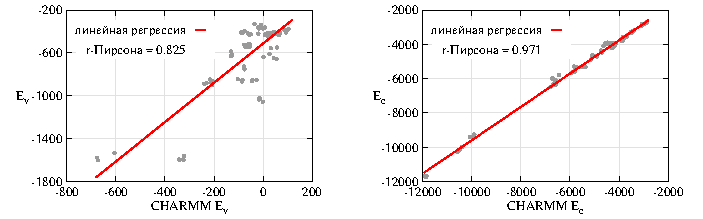
\includegraphics[width=1.0\linewidth]{images/first.pdf}
	\caption{Результаты численного эксперимента для потенциала Леннард-Джонса и для потенциала Кулона}
	\label{first}
\end{figure}

Следует отметить, что представленная на рисунках оценка включает в~себя внутримолекулярные взаимодействия. Для этого в~оценочной функции и~в пакете CHARMM использовалась так называемая схема~1-3, где при формировании списка взаимодействующих пар атомов исключаются пары, которые связаны ковалентно~(схема~1-2), а~также пары, <<соединенные>> одним общим атомом. При рассмотрении компонент комплекса в~виде <<твёрдых>> тел внутримолекулярные взаимодействия изменяться не будут, поэтому при моделировании процесса образования комплекса достаточно выполнить их оценку только один раз и~затем рассматривать взаимодействия только между атомами компонент комплекса.

\begin{figure}[ht!]
	\centering
	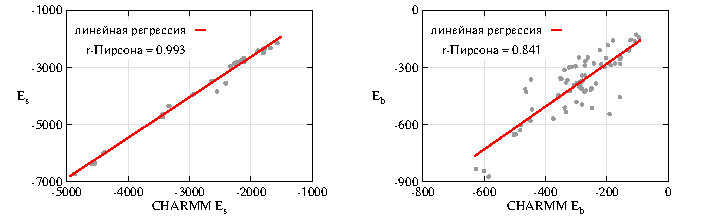
\includegraphics[width=1.0\linewidth]{images/second.pdf}
	\caption{Результаты численного эксперимента для неявного растворителя и для оценки энергии связывания}
	\label{second}
\end{figure}

В простейшем случае процесс связывания описывается моделью вида ключ-замок, которая представляется в~виде $A+B\leftrightarrow AB$, где $A$ и~$B$ являются компонентами комплекса. С~помощью разработанной целевой функции возможно оценить энергию этого взаимодействия. На рисунке~\ref{second} продемонстрирована оценка энергии связывания без учета растворителя, которая определяется по следующей формуле:
\begin{equation}
	E_{b}=\left[E_{v}^{AB} + E_{c}^{AB}\right] - \left[E_{v}^{A} + E_{c}^{A} + E_{v}^{B} + E_{c}^{B}\right].
	\label{bind}
\end{equation}

В численном эксперименте в~начальном PDB файле представлен образованный комплекс $AB$. При определении энергии связывания~\eqref{bind} вычисляется разница между оценкой энергии комплекса в~связанном состоянии и~оценками энергий в~свободном состоянии для каждого компонента в~отдельности. В данном случае оценка энергии растворителя исключена для сравнения результатов оценки взаимодействия только на основе двух слагаемых оценочной функции.